\section{Barcode}
The barcode is a visual representation of the amount of plagiarism in each page of the target document. In our application it is used in two representations, which use the same data source but have another visual layout and details shown within.

\textbf{Real-time data as source}

As the data source we are using real-time data of the document. The data array being generated basically consists of elements with the page number as the key and the percentage of plagiarism as value. That means two resources are included, on the one hand the document pages and on the other hand the fragments on each of these pages.

In the beginning we decided to calculate the percentage of plagiarism for the barcode, whenever the barcode was requested by a user. Although when we had multiple barcodes of large documents on the home page, it turned out to get very slow loading this page. So we limited the data gathering to an update of a fragment or page in the document, the two sources the barcode relies on. This allows us to have the data in real-time, but the calculation of the data does not have to be done on each request and can be cached until the data base changes.

\textbf{Scalable Vector Graphics (SVG) for representation}

Since Unplagged is a web-based project and we are relying on modern techniques as HTML5 and CSS3, we decided to rely on SVG support of the browser as well. This format does have the advantage that it allows building beautiful graphics on the fly that can be changed dynamically and do not require any server resources to be generated, since the generation is being done on the client-side and we can make the graphic dynamically responding to the users browser width. The following code snippet shows the markup for a two bars barcode, each of a 50 percent width and a height of 100 pixels.

\begin{lstlisting}[caption=Barcode SVG markup]
<svg xmlns="http://www.w3.org/2000/svg" version="1.1" style="width: 100%; height: 100px;">
<rect x="0%" y="0" width="50%" height="100" style="fill:#000000;"></rect>
<rect x="50%" y="0" width="50%" height="100" style="fill:#f80012;"></rect>
</svg>
\end{lstlisting}

The barcode can contain up to 5 different colors, which represent the amount of plagiarism within the page:

\begin{itemize}
\item      light blue: the page is disabled for the barcode
\item      white: page not available or no plagiarism
\item      black: more than 0 percent plagiarized
\item      dark red: more than 50 percent plagiarized
\item      light red: more than 75 percent plagiarized
\end{itemize}

As mentioned above, the barcodes can be ouput in two different representations, these will be described below.

\textbf{Representation with labels, used on the home page}

The first representation can be found at the home page, here are the barcodes of all published cases being displayed. The barcode is shown with page numbers below and the width is dynamic, so the barcode increases when the browser width gets bigger and the barcode gets smaller, when the browser width decreases, automatically.

\begin{figure}[!h]
  \centering
  \fbox{
    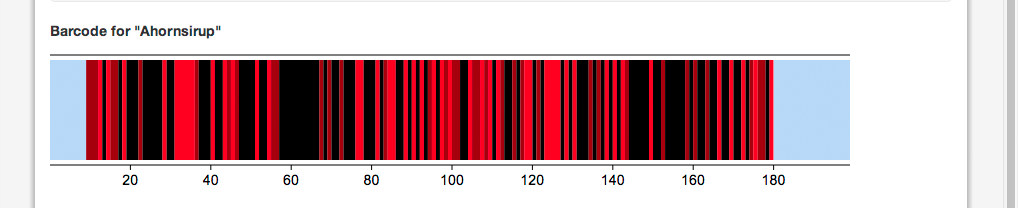
\includegraphics[width=0.97\textwidth]{images/feature-barcode-website.png}
  }
  \caption{Barcode on home page}
  \label{fig:feature-barcode-website}
\end{figure}

Since this mechanism is very dynamic, an algorithm needed to be developed to calculate the x axis values, taking into consideration the page width and the number of pages in the document being visualized. It assumes that a label needs at least 45px of width and the whole barcode has to look well to a minimum width of 500px.

So what we do is, we start with a stepsize of 10 for the page numbers: 10 20 30 40 50, now we check if the amount of pages can be displayed with such a fine scale to stay in the 500px range. For example a page count of 200 leeds to 20 values on the x axis (200 / 10) and if we assume 45px are necessary to display a value on the axis properly, we would need 900px of width, but we have only 500px available. Otherwise we would have crossovers of the labels when we are getting below 900px. So the stepsize is increased by 10, until we stay in the 500px maximum width. As it turns out, a step size of 20 pages is sufficent to get a width of 450px in the end. The code below shows this calculation.

\begin{lstlisting}[caption=Generating the barcode x axis]
private function generateAxis() {
        $labelStepsize = 10;

        while (true) {
            $count = sizeof($this->pages);
            $labelCount = floor($count / $labelStepsize);

            // we assume a label needs 45px and 500px is the width that needs to be displayable without crossovers
            if (45 * $labelCount > 500) {
                $labelStepsize += 10;
                continue;
            }
            break;
        }

        $label = $labelStepsize;
        $x = 0;
        while ($x < ($this->width - ($this->initWidth * $labelStepsize))) {
            $x += ($this->initWidth * $labelStepsize);
            $this->result .= '<text x="' . $x . $this->widthUnit . '" y="' . $this->y . '" font-family="Arial" font-size="14" text-anchor="middle">' . $label . '</text>';
            $this->result .= '<line x1="' . $x . $this->widthUnit . '" y1="' . ($this->y - 20) . '" x2="' . $x . $this->widthUnit . '" y2="' . ($this->y - 15) . '" stroke-width="1" stroke="#000000"></line>';

            $label += $labelStepsize;
        }
    }
\end{lstlisting}

\textbf{Representation without labels in the report}

The second area where barcodes are used, are the final reports, which will be explained in the next section. Since the space available in the PDF is much less than on the website and the library we are using for generating the PDF report does not support text in scalable vectors graphics, we decided to display the barcodes without labels for now. However the data visualized is exactly the same.

\begin{figure}[!h]
  \centering
  \fbox{
    
\includegraphics[width=0.97\textwidth]{images/feature-barcode-report.png}
  }
  \caption{Barcode in the report}
  \label{fig:feature-barcode-report}
\end{figure}

